Les objectifs de ce second hands-on sont:
\begin{itemize}
	\item[-] De se familiariser avec la notion de réponse en fréquence d'un circuit.
	\item[-] De comprendre et de pouvoir interpréter un diagramme de Bode, représentant graphiquement le comportement en fréquence d'un circuit.
	\item[-] De comprendre le fonctionnement et d'implémenter des filtres passe-bas et passe-haut passifs, et d'observer leur impact sur le signal audio.
\end{itemize}
\vspace{.25cm}

\begin{figure} [!ht]
	\centering
	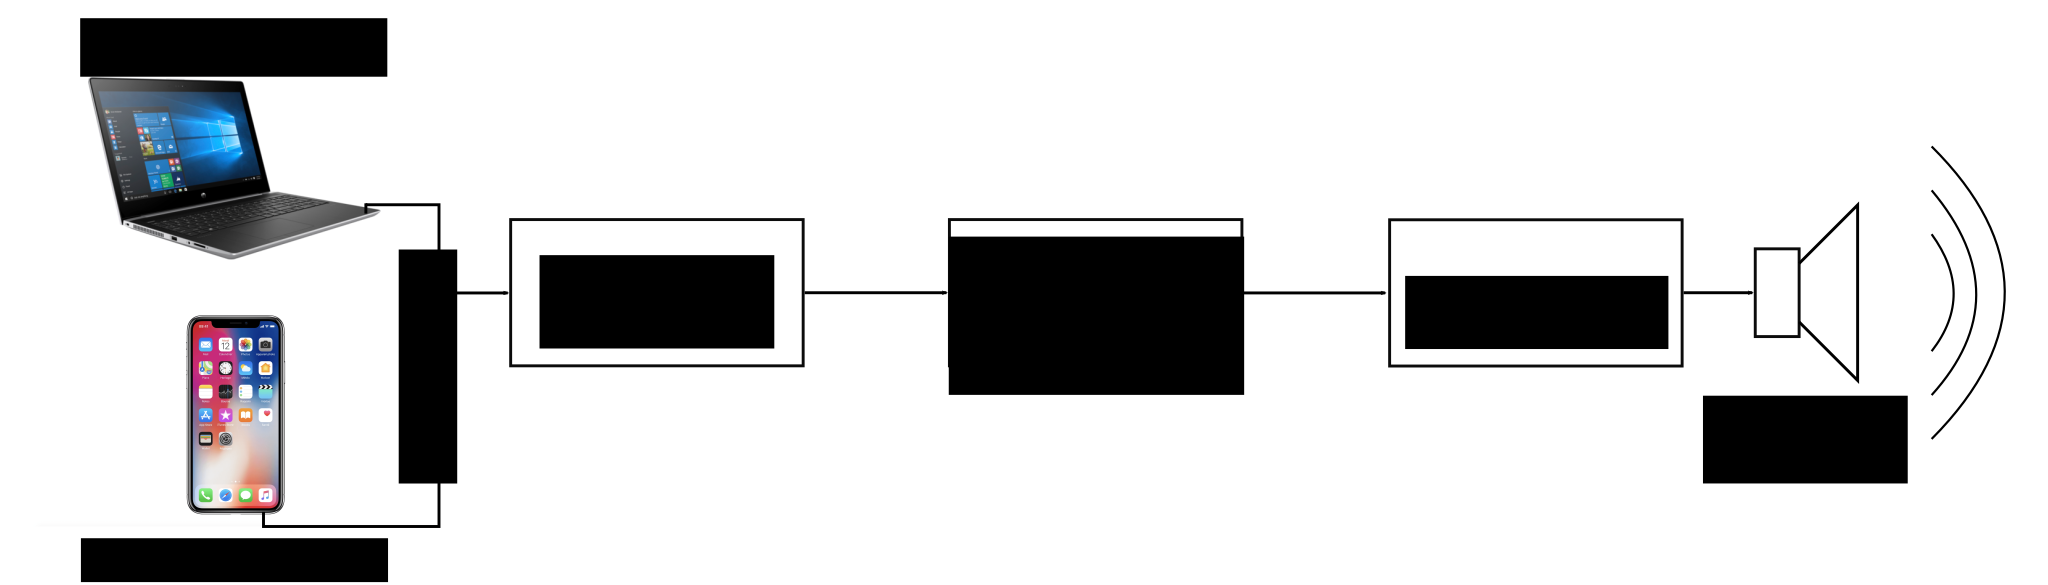
\includegraphics[width=.95\textwidth]{block-diagram}
	\caption{Schéma-bloc du circuit, avec ajout du bloc de filtrage.}
	\label{fig1:block-diagram}
\end{figure}

Le schéma-bloc du circuit modifié est présenté à la Figure \ref{fig1:block-diagram}. En comparaison avec la version proposée lors du premier hands-on, on constate maintenant la présence d'un bloc de filtrage entre le contrôle du volume et l'amplification. Ce bloc va permettre de sélectionner la bande de fréquences destinée à être émise. A titre d'information, la plage de fréquences audibles par l'oreille humaine est comprise entre 20 Hz et 20 kHz.